\chapter{State of Art}
Bevor diese Arbeit auf die Systemarchitektur eingeht, werden hier einige Grundlagen erklärt, die für das Verständnis wichtig sind und über Projekte, die entwickelt wurden. Beginnend werden die verschiedenen möglichen Sensorentypen beschrieben, die mit solch einem Datenhandschuh ausgestattet werden können, wie diese funktionieren und vergleiche sie miteinander. 
Anschließend wird der Datenhandschuh der vorherigen Ausarbeitung vorgestellt und weiter Projekte mit ähnlichen Zielsetzungen.

\section{Sensortypen}
Zur Ermittelung von Bewegung oder Position eines Körperteiles gibt es einige verschiedene mögliche Arten von Sensoren. Abhängig vom Projekttypen können diese individuell verwendet werden, sie haben Vor- und Nachteile die bei bestimmten Projekten hilfreich seien können. Um diese sich genauer zu betrachten, werden sie im folgenden Beschrieben, welche Besonderheiten diese haben und werden zum Schluss Verglichen.

\subsection{Flexion Sensor}
Die Flexion Sensoren sind Sensortypen die sich Daten aus dem zusammen oder auseinander spreizen von Körperteilen oder auch das erweitern von Oberfläche holt. Diese werden typischerweise aus einer Faser gebaut, welches mit einem Detektor und einer LED quelle an den Enden bestattet ist. Durch das bewegen dieser Faser wird mehr Licht zugelassen oder auch geschwächt. Es kann in zwei Arten unterteilt werden, Kopplungsverlustsensor und Biegeverlustsensor \parencite{datagloveForConsumerApplication}.
\begin{center}
\textbf{Kopplungsverlustsensor}
\end{center}
Der Kopplungsverlustsensor ist das Messen von Flächenerweiterung von Körperteilen, die Daten aus dem einknicken des Fingers entnehmen. Diese Art des Sensors besitzt an der LED quelle einen befestigtes Rohr, durch die Oberflächenspannung, die beim Einknicken der Finger entsteht, wird die LED quelle, die Licht durch das Faserteil aussendet, verringert.
\newpage
\begin{figure}[h]
	\centering
    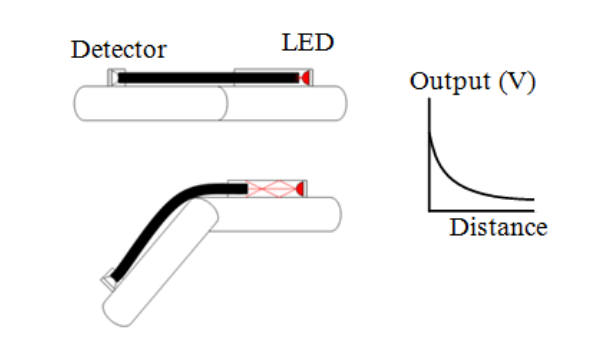
\includegraphics[height=100pt]{Bachelorarbeit/images/FlexionSensor.png}
    \caption{Typ I Flexsensor mit Verwendung einer Faser welches den Kopplungsverlust ermittelt, nach Dataglove for consumer applications (2011)}
    \label{fig:Kopplungsverlust}
\end{figure}
\bigskip
Der Abstand zwischen Licht und Faser erhöht sich und der Detektor empfängt somit weniger Licht. Mit dieser Messung kann das Krümmen der Finger ermittelt werden, welches auch den Krümmungswinkel mit berechnen kann. Je stärker der Finger gekrümmt ist, desto niedriger ist der Lichteinfluss.



\begin{center}
\textbf{Biegeverlustsensor}
\end{center}
Biegeverlustsensor misst den Licht eintritt der LED Quelle durch das spreizen der Finger in das Faserteil, dieses besteht aus einer ungemantelte PMMA-Faser. Hierbei wird der Sensor gebogen zwischen zwei Finger angebracht, welches durch die Krümmung dieser wenig Licht durchlassen. 
\begin{figure}[h]
	\centering
    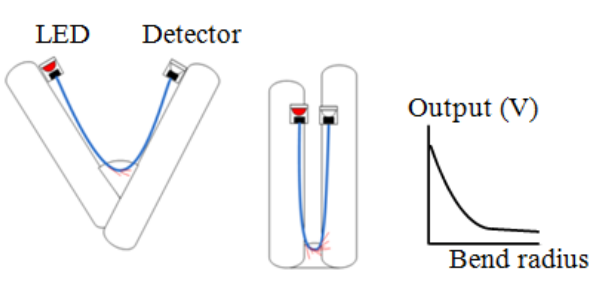
\includegraphics[height=100pt]{Bachelorarbeit/images/BendingLoss.png}
    \caption{Typ II durch das spreizen verringert sich die Biegung und das Licht leuchtet stärker in den Detektor, nach Dataglove for consumer applications (2011)}
    \label{fig:BendingLoss}
\end{figure}
\bigskip

Beim Auseinanderspreizen der Finger wird die Lichtquelle durch die Faser in Richtung Detektor erhöht \ref{fig:BendingLoss}. Die Faser wird typischerweise durch eine starke Biegung sehr belastet und kann sich bei längerer Benutzung auf die Genauigkeit auswirken. 
Diese Art von Sensor erlaubt es uns leider nur einen DoF zu bestimmen, da nur ermittelt wird ob die Faser gebogen oder gestreckt wird.



\subsection{Kamerabasiertes Tracking}
Das kamerabasierte Tracken ist eine Methode, welche zu Beginn Schwierigkeiten hatte im Bereich des Datenhandschuhes fuß zu fassen. In den frühen 1980er baute eine Gruppe der MIT Architecture Machine Group \parencite{ASurveyOfGlove-basedInput} einen Kamerabasiertes LED Tracking um die Körperposition oder eines Körperteils in Echtzeit zu bestimmen. Der Handschuh wurde mit mehreren LEDs ausgestattet und mit der Kamera fokussiert \ref{fig:MITLED}. Der Handschuh war ausschließlich für die Bewegungsaufnahme und nicht Kontrollgeräte verwendet.

\begin{figure}[h]
	\centering
    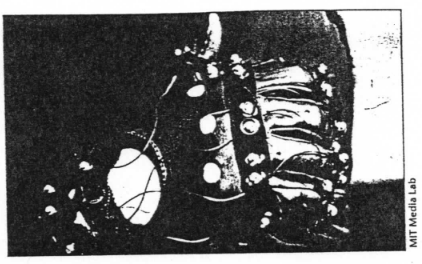
\includegraphics[height=100pt]{Bachelorarbeit/images/MITLED.png}
    \caption{MIT LED Handschuh, entwickelt an der MIT Media Lab in den frühen 1980er}
    \label{fig:MITLED}
\end{figure}
\bigskip

Das Tracken der Handbewegung mit einer kamerabasierten Methode verläuft häufig in einer bestimmten Sequenz. Zu Beginn wird die Hand abfotografiert aus einer Perspektive oder als 3D Modell aus mehreren Perspektiven. Diese Abbildungen werden mit bestimmten Programmen analysiert und bewertet, die Finger werden aus dem Modell bestimmt durch komplexe und gesetzte Bildverarbeitungsmethoden. Aus diesem Verfahren werden dann die Fingerposition, sowie andere gefragte Daten ausgegeben.

\subsection{IMU - Insertial Measurement Unit}
Inertial Measurement Units sind Sensoren die in der Lage sind verschiedene Messdaten der unterschiedlichen Bewegungsrichtungen zu messen. Diese Messdaten bestehen häufig aus der linearen Beschleunigung, die Winkelgeschwindigkeit und einem Kompass, sie messen gewöhnlicherweise 3 DoF, also den Degree of Freedom oder auch Freiheitsgrad.\parencite{Reviews} Dafür verwenden viele Modelle üblicherweise das MEMS System, Mikroelektromechanisches System, das sind Bauteile die für den jeweiligen DoF eine bestimmte Funktion besitzt.
\begin{figure}[H]
    \centering
    \subfloat[Beschleunigungssensor]{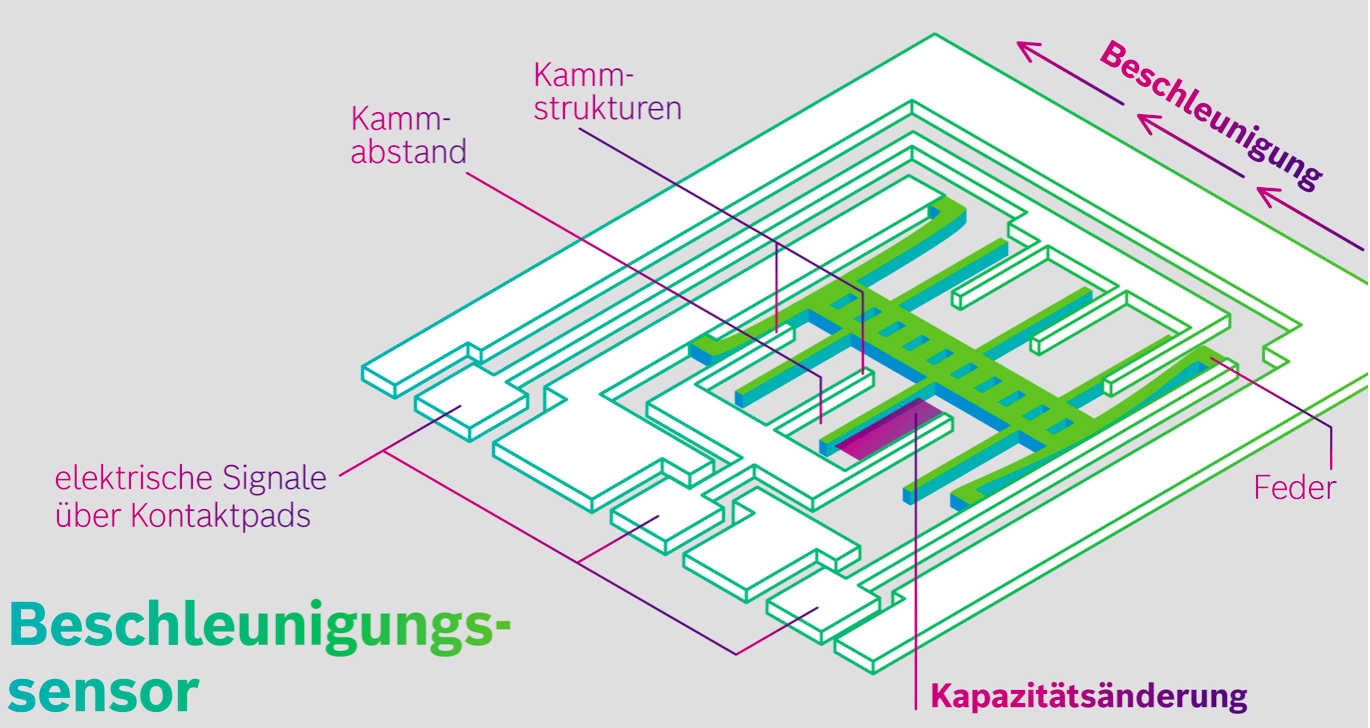
\includegraphics[width=0.31\textwidth]{Bachelorarbeit/images/MEMSBeschleunigung.png}\label{Beschleunigung}} 
    \subfloat[Gyroskope]{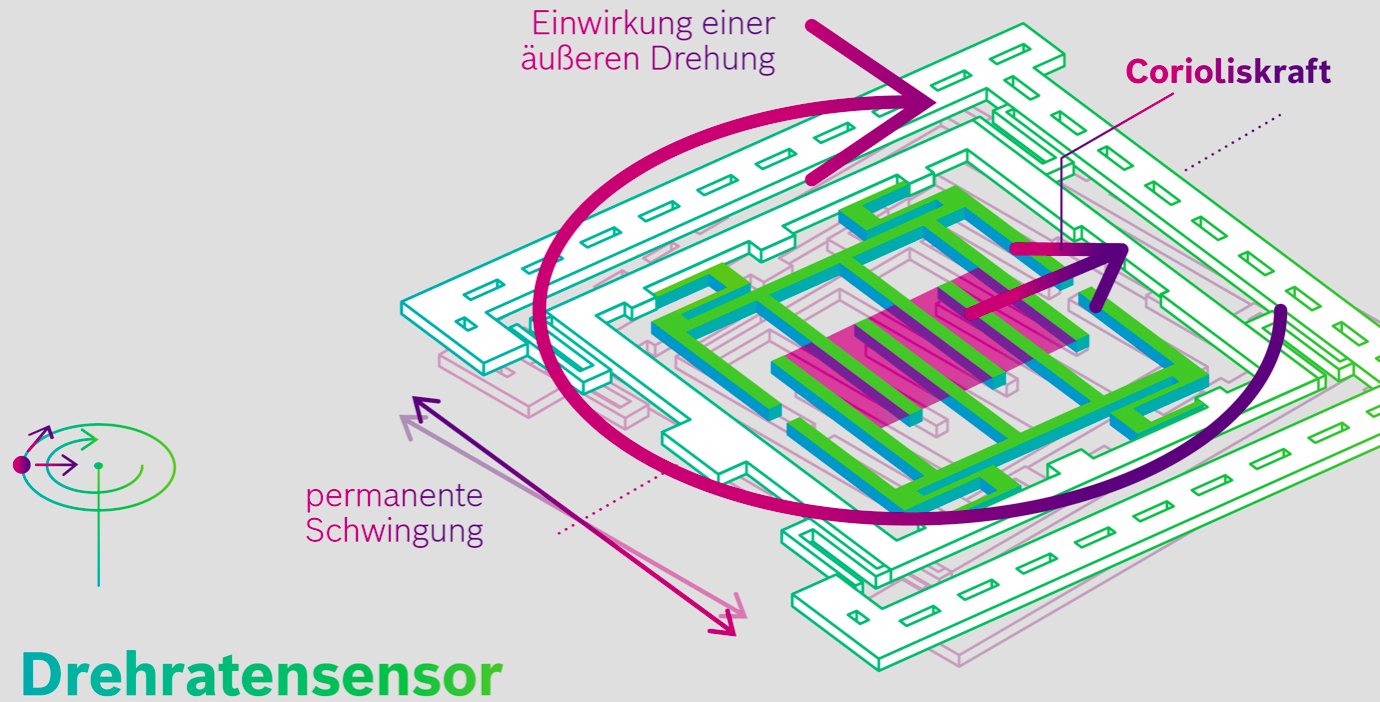
\includegraphics[width=0.31\textwidth]{Bachelorarbeit/images/MEMSGyroskope.png}\label{Gyroskope}} 
    \subfloat[Magnetometer]{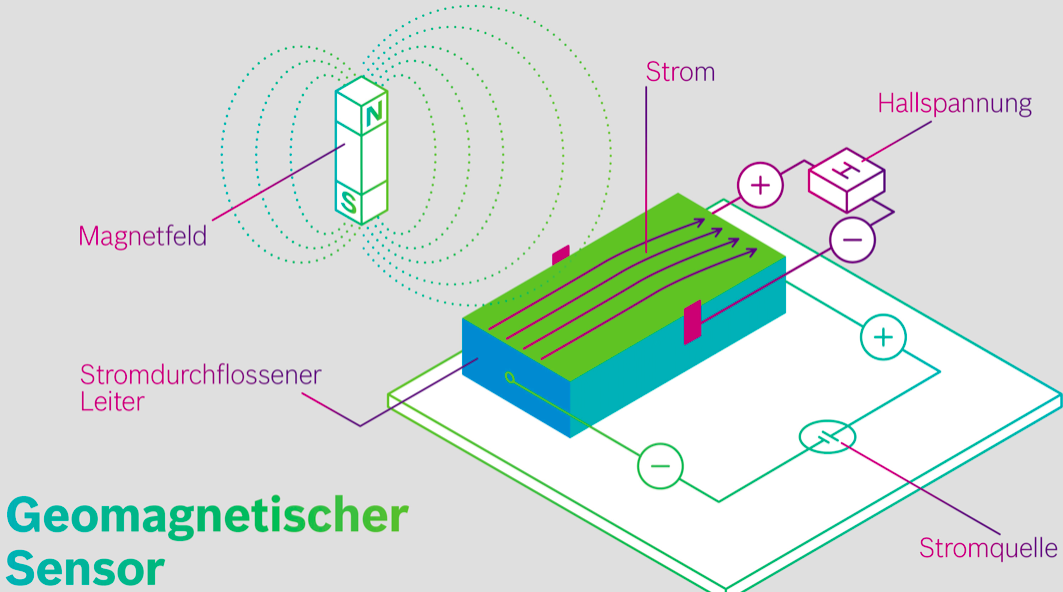
\includegraphics[width=0.31\textwidth]{Bachelorarbeit/images/MEMSMagnetometer.png}\label{Magnetometer}} 
    \caption{Illustrationen des MEMS-Systeme von der Bosch GmbH}
    \label{fig:BoschFigures}
\end{figure}

Die lineare Beschleunigung\protect\subref{Beschleunigung} verwendet in den MEMS Systemen eine Kammstrukturen die mit Federung an elektrischen Kontaktpads verbunden sind, jedoch besteht zwischen der Kammstruktur und den Kontaktpads ein gewisser Kapazitätsabstand. Bei Beschleunigung wird die Kammstruktur abgefedert und es eine entsteht eine Kapazitätsänderung, mit dieser Veränderung wird somit die Beschleunigung gemessen.\parencite{web:BoschBMI}
\\
Das MEMS System für die Winkelgeschwindigkeit\protect\subref{Gyroskope} verwendet das Prinzip der Corioliskraft, welches wenn Drehungen auf das Modull ausgeübt wird, die Kammabstände innerhalb der Kammstruktur ihre Abstände verändert, welche somit zur Änderung der Kammkapazität führt.\parencite{web:BoschBMI}
\\
Die Kompass Funktion des MEMS\protect\subref{Magnetomete} verwendet das Prinzip von Hall, welches bei einem durchfließenden Leiters in einem homogenen Magnetfeld, senkrecht zu beiden Leitern eine Spannung erzeugt, die Hall-Spannung. Mit diesem Prinzip ist es somit möglich die Magnetfelder zu messen und Kompass Koordinaten auszugeben.\parencite{web:BoschBMI}


\section{Vergleich}
Diese drei Arten von Sensorentypen haben alle unterschiedliche Vor- und Nachteile. 
Abhängig vom Material, Kostenplan, Verwendungszweck und der Ausführungsmethode, gibt es immer verschiedene Lösungswege um Positionen und Bewegungsabläufe zu bestimmen, von Körperteilen oder auch Objekten.
\begin{itemize}
    \item Der Flexion Sensor kann durch sehr simples Material gebaut werden, jedoch hängt diese Genauigkeit auch von der Qualität ab. Die Handgröße spielt auch eine große Rolle für die Konsistenz der Daten, den verschiedene Größen können den Nutzer falsche Daten geben. Eine gute Kalibrierung kann auch viel Zeit in Anspruch nehmen, dabei kann es schon mal Stunden dauern, für eine gewisse Handgröße, jedoch kann diese anschließend gespeichert und nach bedarf abgerufen werden.
    
    \item Das kamerabasiert Tracking ist das registrieren der Hand Position, hierfür ist lediglich eine Kamera notwendig, um die Hand oder ein Objekt zu erfassen. Kameras sind derzeit billig auf dem Markt, was es, wenn es um die Kosten geht ein Vorteil bringt. Kalibrierung ist schnell, da bei Verwendung die Kamera Position und die Knochenlänge wichtig sind, beides kann während des Bildverarbeitungprozess ermittelt werden. Leider ist die Genauigkeit der Daten sehr anfällig, denn bei qualitativ schlechteren Kameras kann bei schneller Bewegung ein Motion Blur entstehen; eine Bewegungsunschärfe, welches somit die Genauigkeit gänzlich verfehlt. Bei der Konsistenz kann es auch sehr problematisch werden, wenn eines der Finger bedeckt oder dem falschen Finger zugeordnet wird, bei diesen Situationen sind die Daten häufig obsolet.
    
    \item IMUs können beim tracken jedes einzelnen Gelenks sehr teuer werden, jedoch reichen häufig nur einige Module aus, die beispielsweise an den Fingerkuppen und der Mittelhand befestigt werden können. Die Genauigkeit der Daten hängt von der Qualität und der Kalibrierung des IMUs ab, dabei kann die Kalibrierung unterschiedlich lange dauern, das ist abhängig vom Bedarf der Genauigkeit. Zwei Arten der Kalibrierung werden dabei verwendet, die Standard Kalibrierung, bei der nur ein IMU gemessen wird oder die Kreuz-Kalibrierung, in welcher der relative Winkel von mehreren IMUs bestimmt werden, wobei die Änderung eines wertes einer einzelnen IMU Kalibrierung die komplette Kreuz-Kalibrierung nicht mehr gebräuchlich macht.
\end{itemize}
Im Vergleich steht der IMU mit seinen Qualitäten besser, da dieser es erlaubt Beschleunigungs und Winkelgeschwindigkeit zu messen, wird nicht durch die äußere Umgebung beeinflusst, ausgenommen das Modul besitzt einen Magnetometer, denn hier könnte durch fremde Magnetwellen die Daten verfälscht werden und sind auch kostengünstig in Maßen. Im Gegensatz zu dem kamerabasierten Tracking, werden die Rohdaten ohne jegliche Bildverarbeitung und gut platzierter Kamera erzeugt und können durch Sensorfusion auch stabilere Daten ausgeben. Flexion Sensoren sind einfacher in der Messung von Daten, jedoch sind diese limitiert auf 1 DoF und bei komplexeren Gelenken mit mehreren Bewegungsrichtungen reicht dieser häufig nicht aus. Zum erstellen eines Datenhandschuhes ist es wichtig zu wissen welche Gelenke gemessen werden, welche Materialien zu Verfügung stehen und wie genau die Daten gemessen werden sollen. Um akzeptable Daten für die Hand zu bekommen, wurde beschlossen die Finger und die Handfläche zu bestimmen. Der Freiheitsgrad vom Zeigefinger bis zum Kleinen Finger liegt bei 2 DoF \parencite{gloveBasedSystems}, wobei der Daumen und die Handfläche in alle drei Richtungen bewegt werden können, das spricht für Verwendung des IMU Sensors. Für all diese Freiheitsgrade müssten mehrere Flexion Sensoren angebracht werden, welches sehr unübersichtlich werden kann, wobei die IMUs mit einem Modul 3 DoF abdeckt. Das kamerabasierte Tracking fällt durch die statische Kameraposition und deren limitierten Sichtweite aus, da dieses System von der Mobilität und Position unabhängig bleiben soll.\parencite{Wokke}


\section{Alternative Datenhandschuhe}\label{alternativeDatenhandschuhe}
Im folgenden werden zwei alternative Datenhandschuhe vorgestellt, welche im aktuellen Stand der Technik weit ausgeprägt sind, der Manus Prime II und der BeBop Forte Data Glove. 
\\
\\
\begin{center}
\textbf{Manus Prime II}
\end{center}
Der Manus Prime II \parencite{web:ManusPrimeII} wurde hauptsächlich zum Motion Capture und der virtuellen Realität entwickelt. Dieser ist mit jeder VR-Applikation, sowie mit wichtigen Plugins für Unity,Unreal Engine oder Autodesk Motionbuilder kompatibel. Die Bewegung der Finger werden durch 16 Sensoren gemessen, diese bestehen aus 10 Flexion Sensoren die pro Finger zwei Gelenke messen und aus sechs IMUs mit 9 DoF, für die detaillierte Messung der Finger. Der integrierte Akku erlaubt die drahtlose Benutzung bis zu fünf Stunden störungslose Motion Capture. Durch die Konstruktion ist die Batterie in der Lage während des Aufladen noch in der Verwendung zu bleiben, jedoch falls ein wechsel der Batterie notwendig ist kann dieser problemlos gewechselt werden. Die Frequenz von dem Manus Prime II liegt bei 90 Hz, die Genauigkeit varriert zwischen +-2,5 Grad und hat ein Gewicht von 60 Gramm. Dieser Datenhandschuh ist durch seine komplexe Datenmessung und seiner allgemeinen Funktion, wie der hohen Frequenz, drahtlosen Verwendung oder der einfachen Verbindung zu gegebenen Applikationen ein sehr Fortgeschrittener Handschuh.
\\
Die Systemintegration läuft über die eigene Applikation, diese wird direkt über den Ressource Center heruntergeladen und hilft dem Benutzer bei der Kopplung des Produktes.
Das einleiten der Daten verläuft über den Manus Dongle, der direkt an den PC angeschlossen wird und kommuniziert dann mit der Applikation. Das Handschuhpaar ist schon auf den Manus Dongle vorkonfiguriert. Dieser erhält dann die Daten von dem Handschuh paar und übermittelt die Werte an die Applikation weiter. Anschließend für genauere Messungen kann dieser kalibriert werden, welche 30 Sekunden dauert und auf das System abgespeichert wird.
\begin{figure}[h]
	\centering
    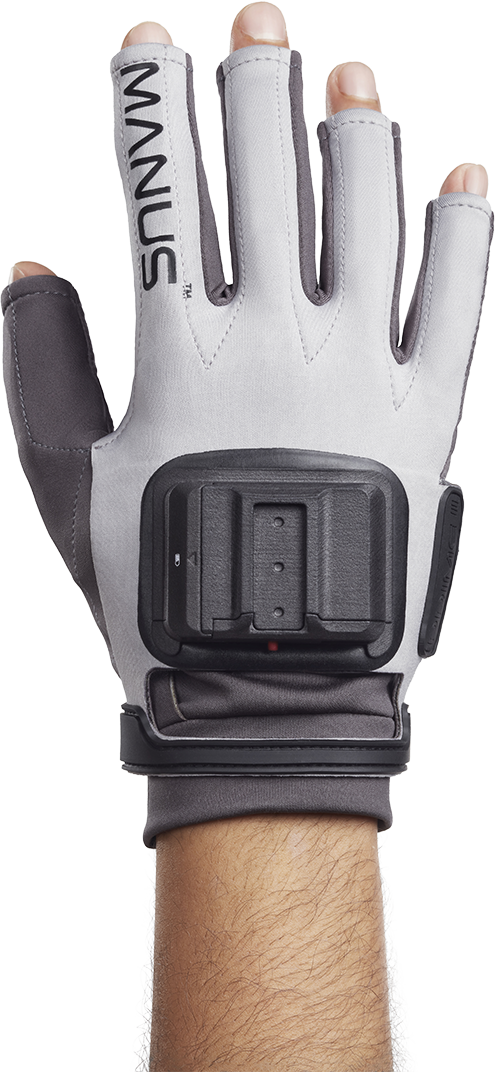
\includegraphics[height=200pt]{Bachelorarbeit/images/ManusPrimeII.png}
    \caption{Manus Prime II}
    \label{fig:ManusPrimeII}
\end{figure}
\\
\\
\begin{center}
\textbf{Forte Data Glove}
\end{center}
Forte Data Glove \parencite{web:BeBoP} ist eine, von BeBop Sensors entwickelter Datenhandschuh, welcher mit einer hohen Leistung und haptischer Funktion gebaut wurde. Der Anwendungsbereich liegt in der AR/VR Domäne und kommuniziert durch USB oder Bluetooth Verbindung. Genau wie der Manus Prime II verwendet dieser auch insgesamt 16 Sensoren, mit der gleichen Verteilung von Flexion Sensoren und IMUs. Der Forte Data Glove erlaubt nicht nur Messung der Hand und Finger Bewegung, sondern auch eine haptische Rückmeldung, welche aus den benutzerdefinierten nicht resonanten Aktuatoren produziert wird, befestigt an den Fingerspitzen und der Handfläche. Mit der Verarbeitung der Flexion Sensoren, IMUs und der haptischen Rückmeldung läuft dieses Produkt mit einer Frequenz von 200 Hz und einer Latenz von 150 fps. Durch seine integrierte Lithium Polymer Batterie erlaubt dieser eine drahtlose Benutzung von zwei Stunden.
\\
Der Forte Glove kann über zwei Wege an das Host System verbunden werden, über direkte Verbindung mit dem USB-C Kabel oder die Bluetooth Funktion. Für die Bluetooth Funktion wurde ein spezieller USB Stick entwickelt, welcher direkt an den PC angeschlossen wird und den es dem Nutzer erlaubt sich darüber zu verbinden. Für die Kopplung kann ein Treiber installiert werden, der mit der Verbindung aus hilft, jedoch in den meisten Fällen haben die Programme, wie Unity oder Unreal Engine installierbare Plugins, mit denen der Handschuh sich verbinden kann. 
\begin{figure}[h]
	\centering
    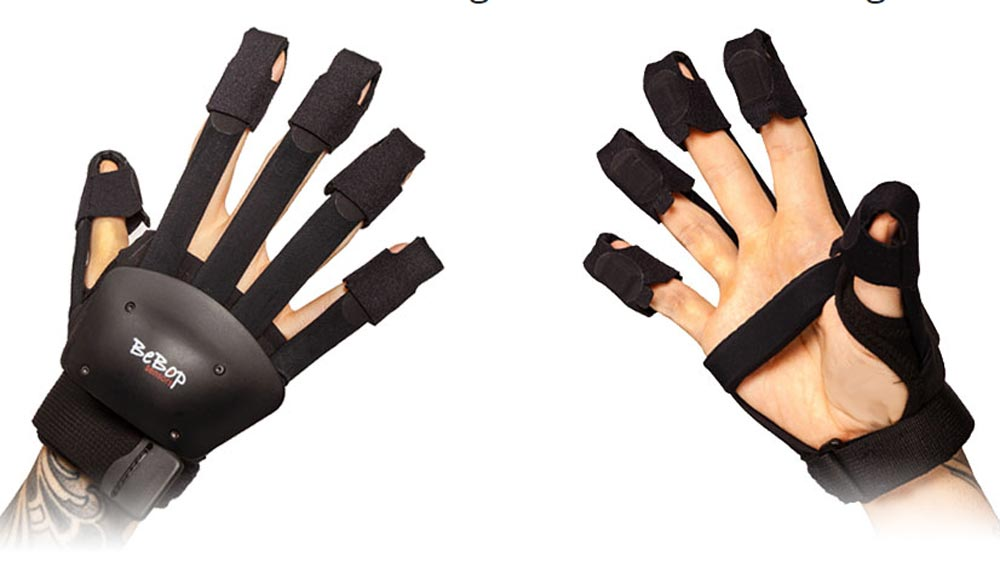
\includegraphics[height=200pt]{Bachelorarbeit/images/bebop_handschuh.jpg}
    \caption{Forte Data Glove}
    \label{fig:ForteDataGlove}
\end{figure}
\\
\\
Diese kommerziellen Datenhandschuhe sind fortgeschritten und für den Markt tauglich, durch ihre hohe Frequenz und ihrer stabilen Systemarchitektur gehören diese zu Vorbildern für zukünftige Datenhandschuhe.  